\section{Analysis on Weight Difference before and after COVID-19}

In this section, we aim to investigate if the COVID-19 situation had any impact on the weight of individuals. The study involved collecting data from 230 individuals, and the subsequent analysis is based on this dataset.

Consider paired data $(X_{1}, Y_{1}), \ldots, (X_{n}, Y_{n})$ representing the weights of $n$ individuals before and after COVID-19, respectively. Here, $X_{i} \sim \text{IID} \ N(\mu, \sigma^{2})$ represents the weight distribution before COVID-19, and $Y_{i} \sim \text{IID} \ N(\mu, \sigma^{2})$ represents the weight distribution after COVID-19.

Here, 
$$
\begin{aligned}
    E(X_{i}) &= \mu_{1}, \quad V(X_{i}) = \sigma_{1}^{2}, \quad \forall \ i = 1, 2, \ldots, n \\
    E(Y_{i}) &= \mu_{2}, \quad V(Y_{i}) = \sigma_{2}^{2}, \quad \forall \ i = 1, 2, \ldots, n
\end{aligned}
$$
where $\sigma_{1}$ and $\sigma_{2}$ are unknown.

Assuming normality, our goal is to test if the weight remains the same before and after COVID-19 against the alternative hypothesis.

\textbf{Hypothesis}:
$$H_{0} : \mu_{1} = \mu_{2} \ \text{vs} \ H_{1} : \mu_{1} \neq \mu_{2}$$

Here, $(X_{i}, Y_{i}) \sim \text{BVN} (\mu_{1}, \mu_{2}, \sigma_{1}^{2}, \sigma_{2}^{2}, \rho)$, where $\rho$ is the correlation coefficient of $X_{i}$ and $Y_{i}$.

Define $D_{i} = X_{i} - Y_{i}$ for $i = 1, 2, \ldots, n$. The $D_{i}$'s are IID $N(\mu_{1} - \mu_{2}, \sigma^{2})$, where
$$
\sigma^{2} = V(X) + V(Y) - 2 \text{Cov}(X, Y) = \sigma_{1}^{2} + \sigma_{2}^{2} - 2 \rho \sigma_{1} \sigma_{2}.
$$

Now, the hypothesis test becomes equivalent to a one-sample test:
$$H_{0} : \mu = 0 \ \text{vs} \ H_{1} : \mu \neq 0 \ \text{with unknown} \ \sigma^{2},$$
where $\mu = \mu_{1} - \mu_{2}$.

In this two-tailed test, consider
$$\Bar{D} = \frac{D_{1} + \ldots + D_{n}}{n}.$$
Then, $\Bar{D} \sim N(\mu, \frac{\sigma^{2}}{n})$.

\textbf{Test Statistics}:
Consider the following test statistic using a paired t-test:
$$T = \frac{\Bar{D} - \mu}{\frac{s}{\sqrt{n}}},$$
where $s$ is the sample standard deviation. The statistic $T$ follows a $t$-distribution with $(n-1)$ degrees of freedom.

Now, based on the data collected from 231 observations:
$$\text{mean} = \Bar{d} = 3.058696$$
$$\text{median} = m_{e} = 3$$
$$\text{variance} = 45.643920$$
$$\text{standard deviation} = 6.756028$$

Under the null hypothesis $\mu = 0$ and $s = 0$,
$$T = \frac{\Bar{D} \sqrt{n}}{s}.$$

Using the given data, $t = 6.866079$, the observed value of $T$.

\textbf{Critical Region}:
With $n = 230$ and degrees of freedom $= 229$, the critical region at a $5\%$ level of significance is
$$(-\infty , 1.9709] \ \bigcup \ [1.9709, \infty).$$

\textbf{Decision Rule}:
We reject the null hypothesis if the test statistic lies in the critical region. In our case, $t = 6.866079$ lies within the critical region, leading us to reject the null hypothesis $H_{0} : \mu = 0$ in favor of $H_{1} : \mu \neq 0$.

\textbf{Result Interpretation}:
Rejecting the null hypothesis provides strong evidence that there is a statistically significant difference in weights before and after COVID-19. Thus, our study suggests that the COVID-19 pandemic might have had an impact on individuals' weights.

Below is a pictorial representation of the dataset of weight differences (Figure \ref{G39}):

\begin{figure}[h!]
    \centering
    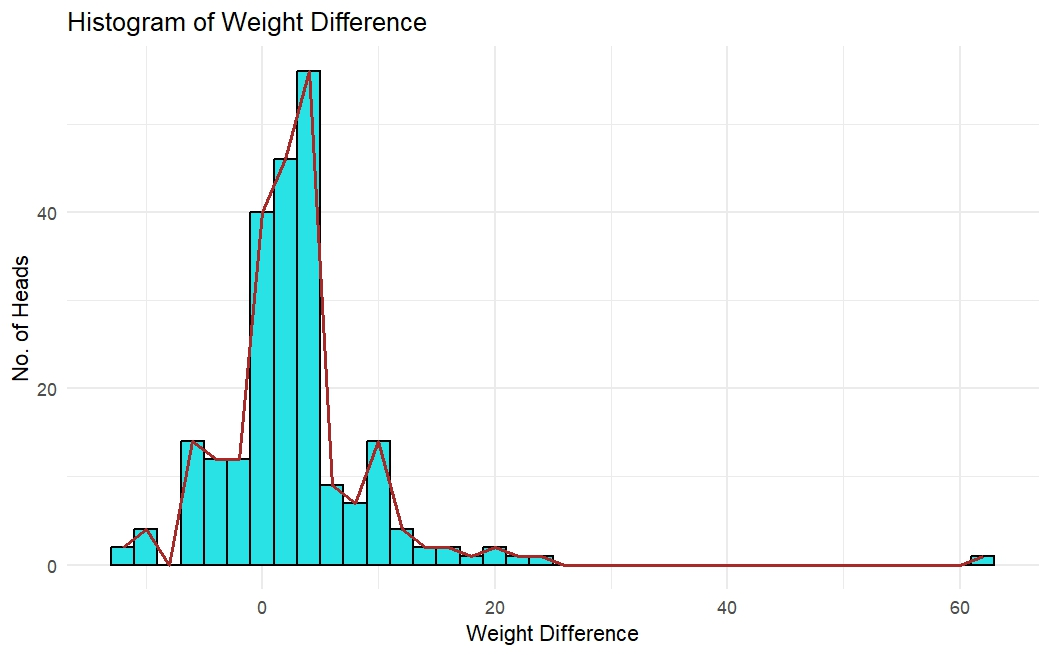
\includegraphics[width=0.7\linewidth]{IMAGES/Image 39.jpg}
    \caption{Difference in Weights}
    \label{G39}
\end{figure}

The graph indicates outliers in the dataset. However, excluding these, the data is clustered between $-20$ to $30$, suggesting that individuals under study may have experienced significant changes in their weights.
